\documentclass[12pt]{exam}

\usepackage[brazil]{babel}   
\usepackage[TS1,T1]{fontenc}
\usepackage[utf8]{luainputenc}
\usepackage[utf8]{inputenc}  
%\usepackage[T1]{fontenc}
\usepackage{amsfonts,amsmath,amssymb,latexsym} 
\usepackage{enumerate}
\usepackage{float}
\usepackage{graphicx}
\usepackage{caption}
\usepackage{subcaption}
\graphicspath{ {images/} }




\def\cQ{\mathcal{Q}}
\def\ve{\varepsilon}

\def\emptyset{\varnothing}
\def\ept{\varnothing}

% Include the listings-package
\usepackage{listings}             
\usepackage{color}

\definecolor{dkgreen}{rgb}{0,0.6,0}
\definecolor{gray}{rgb}{0.5,0.5,0.5}
\definecolor{mauve}{rgb}{0.58,0,0.82}

\lstset{frame=tb,
  language=Prolog,
  aboveskip=3mm,
  belowskip=3mm,
  showstringspaces=false,
  columns=flexible,
  basicstyle={\small\ttfamily},
  numbers=left,
  stepnumber=1,  
  numberstyle=\tiny\color{gray},
  keywordstyle=\color{blue},
  commentstyle=\color{dkgreen},
  stringstyle=\color{mauve},
  breaklines=true,
  breakatwhitespace=true,
  tabsize=3
}


\usepackage{tikz}
\usetikzlibrary{trees}



\usepackage[margin=1in]{geometry}
\usepackage{amsmath,amssymb}
\usepackage{multicol}

\def\code#1{\texttt{#1}}

\newcommand{\class}{IA}
\newcommand{\term}{1º semestre de 2021}
\newcommand{\examnum}{Lista 03}
\newcommand{\examdate}{}

\pointpoints{ponto}{pontos}

\pagestyle{head}
\firstpageheader{}{}{}
\runningheader{\class}{\examnum\ - Página \thepage\ de \numpages}{\examdate}
\runningheadrule


\begin{document}

\noindent
\begin{tabular*}{\textwidth}{l @{\extracolsep{\fill}} r @{\extracolsep{6pt}} l}
\textbf{\class} & \textbf{Nome:} & \makebox[2in]{\hrulefill}\\
\textbf{\term}  & \textbf{RA:}   & \makebox[2in]{\hrulefill}\\
\textbf{\examnum} &&\\
& Professor: & Vinicius Pereira
\end{tabular*}\\
\rule[2ex]{\textwidth}{2pt}

Esta lista contém \numpages\ páginas e \numquestions\ questões.\\


\noindent
\rule[2ex]{\textwidth}{2pt}


\vspace{3em}


\begin{description}

\item[Algoritmo $A$]:\\
Considere a função de avaliação $f(n) = g(n) + h(n)$, onde
  \begin{description}
    \item $n$ é um estado qualquer encontrado na busca
    \item $g(n)$ é o custo de chegar até $n$ a partir do estado inicial
    \item $h(n)$ é a estimativa heurística do custo de ir de $n$ até um objetivo
  \end{description}
Se esta função de avaliação for usada com a heurística de busca pela melhor escolha, o resultado é chamado algoritmo $A$.

\item[Algoritmo $A^*$]:\\
Seja $h^*(n)$ a função de avaliação heurística que retorna o valor exato da distância da melhor solução do vértice $n$ até algum objetivo.\\
Então uma heurística $A^*$ usa uma heurística de avaliação $h(n)\leq h^*(n)$.\\
Note que não temos como saber exatamente $h^*(n)$, só como estimar uma $h(n)\leq h^*(n)$.\\
Então a função de avaliação $f(n)$ de $A^*$ é $f(n) = g(n) + h(n)$, onde $h(n)\leq h^*(n)$.\\

\item[Admissibilidade]:\\
Uma Busca $A$ com heurística de avaliação $f(n) = g(n) + h(n)$, tal que $h(n)\leq h^*(n)$, é uma heurística admissível.\\
Heurísticas admissíveis chegam, eventualmente, na resposta ótima.\\
Note que o Algoritmo $A^*$ é admissível.\\

%\item[Monotonicidade]:\\
%Uma Busca $A$ é uma heurística monotônica se usa como heurística de avaliação $f(n) = g(n) + h(n)$, tal que 
%\begin{description}
%  \item $h(n)\leq c(n, n') + h(n')$, onde $n$ e $n'$ são estados do espaço de estados,
%  \item A avaliação heurística do estado objetivo é $0$, $h(\mbox{Objetivo}) = 0$.
%\end{description}
%Heurísticas monotônicas são admissíveis e sempre encontram o melhor caminho para cada vértice que ela fecha.\\
%

\item[Grau de informação]:\\
Para duas Heurísticas $A^*$, $h_1$ e $h_2$, se $h_1(n)\leq h_2(n)\leq h^*(n)$ para todo vértice $n$, então se diz que a heurística $h_2$ é mais bem informada que a heurística $h_1$.

\end{description}


\break

\begin{questions}


\question Um quebra-cabeça de peças deslizantes consiste em um tabuleiro unidimensional com 7 espaços, três peças pretas no extremo esquerdo, três peças brancas no extremo direto, e um espaço vazio no meio, figura \ref{fig:bp}.

\begin{figure}[h]
    \centering
    
\includegraphics[width=0.60\textwidth]{bp}
    \caption{Quebra-cabeça de peças deslizantes}
    \label{fig:bp}
\end{figure}

Uma peça pode ser movida para uma casa adjacente, este movimento tem custo 1. Uma peça pode pular uma ou duas peças para um espaço em branco, este movimento tem o custo da quantidade de peças puladas.

O objetivo é ter todas as peças brancas a esquerda de todas as peças pretas, a posição do vazio não é importante.

Defina um espaço de estado para o problema.

Use a busca da melhor escolha como heurística de busca e desenvolva \textbf{duas} heurísticas de avaliação.

Argumente se as suas heurísticas de avaliação são admissível e/ou monotônica. Qual tem mais informação?

\break

\question Discuta a admissibilidade
%, monotonicidade 
e grau de informação para as seguintes heurísticas do 8-puzzle:\\
$f(n) = g(n)+h(n)$, onde $g(n)$ é o número de passos dados até chegar em $n$ e $h(n)$ é

\begin{enumerate}
\item O número de peças fora do lugar.
\item A soma da distância de cada peça até o seu lugar objetivo
\item Gere três instâncias do estado $n$. Nas três instâncias o espaço vazio está no mesmo lugar que na instância original; na primeira as três peças de cima são iguais, as outras peças com um símbolo x; na segunda com as três peças do meio (em relação à altura) são iguais, as outras peças com um símbolo x; na terceira as três peças de baixo são iguais, as outras com um símbolo x (um exemplo é visto na figura \ref{fig:8p3heu}). O valor é a soma do menor número de passos para resolver cada um dos três problemas, deixando o espaço vazio no meio, peças com símbolo x em qualquer lugar e peças com números específicos em seus lugares específicos.
\end{enumerate}

OBS: Caso a heurística não seja admissível mostre um contra exemplo. Neste caso você deve criar uma instância que não seja admissível e mostrar.\\
OBS2: Não use o exemplo dado para explicar a heurística, mesmo por que é possível que ele nem tenha solução.



\begin{figure}[h]
    \centering
    \includegraphics[width=0.60\textwidth]{8p3heu}
    \caption{Um exemplo de uma das heurísticas de avaliação.}
    \label{fig:8p3heu}
\end{figure}


\question Considere o problema em que você deve programar um robô para empilhar e desempilhar caixas em uma sala. Considere que na sala existe, pelo menos, três espaços para empilhar as caixas, a altura que a pilha alcança é ilimitada. No estado inicial já existem caixas empilhadas. Cada caixa tem uma identificação. O robô consegue empilhar ou desempilhar uma caixa por vez. O objetivo é do tipo ``Colocar a caixa $X$ logo em cima da caixa $Y$''.

Desenvolva uma heurística de avaliação para uma busca do algoritmo $A$. Discuta se a sua heurística é admissível
% e monotônica
.


\end{questions}

\end{document}

